\subsection{Điều kiện chấp nhận kết luận và luật không đoán}
\label{sec:verdict_acceptance}

Mục này nêu tiêu chí hình thức để Game Engine chấp nhận một phán quyết, cách
quy tiêu chí đó về bài toán SAT, và luật ``không đoán'' mà tiêu chí này bảo
đảm.

\paragraph{Điều kiện suy diễn.}
Phán quyết $\langle i, s\rangle$ được chấp nhận tại thời điểm $t$ khi và chỉ
khi nó là hệ quả logic của tri thức công khai:
\begin{equation}
  \mathit{KB}_t \models (x_i = s)
  \iff
  \mathit{KB}_t \land (x_i \ne s) \text{ không thỏa được}.
  \label{eq:entailment}
\end{equation}
Vế phải của \eqref{eq:entailment} là một truy vấn SAT. Hàm
\texttt{has\_solution(state, assumption)} của bộ kiểm tra trả về
\texttt{True} khi $\mathit{KB}_t$ cùng giả thiết tùy chọn thỏa được. Game
Engine gọi hàm này hai lần,
\begin{equation}
  a = \mathrm{SAT}\bigl(\mathit{KB}_t \land (x_i = s)\bigr),
  \qquad
  b = \mathrm{SAT}\bigl(\mathit{KB}_t \land (x_i \ne s)\bigr),
\end{equation}
và phân loại kết quả theo cặp $(a, b)$. Truy vấn $a$ là cần thiết dù
\eqref{eq:entailment} chỉ dùng $b$: nó tách trường hợp phán quyết bị bác bỏ
khỏi trường hợp chính $\mathit{KB}_t$ mâu thuẫn.

\paragraph{Phân loại kết quả.}
Hình~\ref{fig:verdict_outcome} mô tả thứ tự kiểm tra trong
\texttt{submit\_verdict}, và Bảng~\ref{tab:submit_outcome} liệt kê sáu kết quả
có thể. Chỉ kết quả \texttt{ACCEPTED} làm thay đổi trạng thái ván chơi; năm kết
quả còn lại trả về ảnh chụp công khai không đổi.

\begin{figure}[htbp]
  \centering
  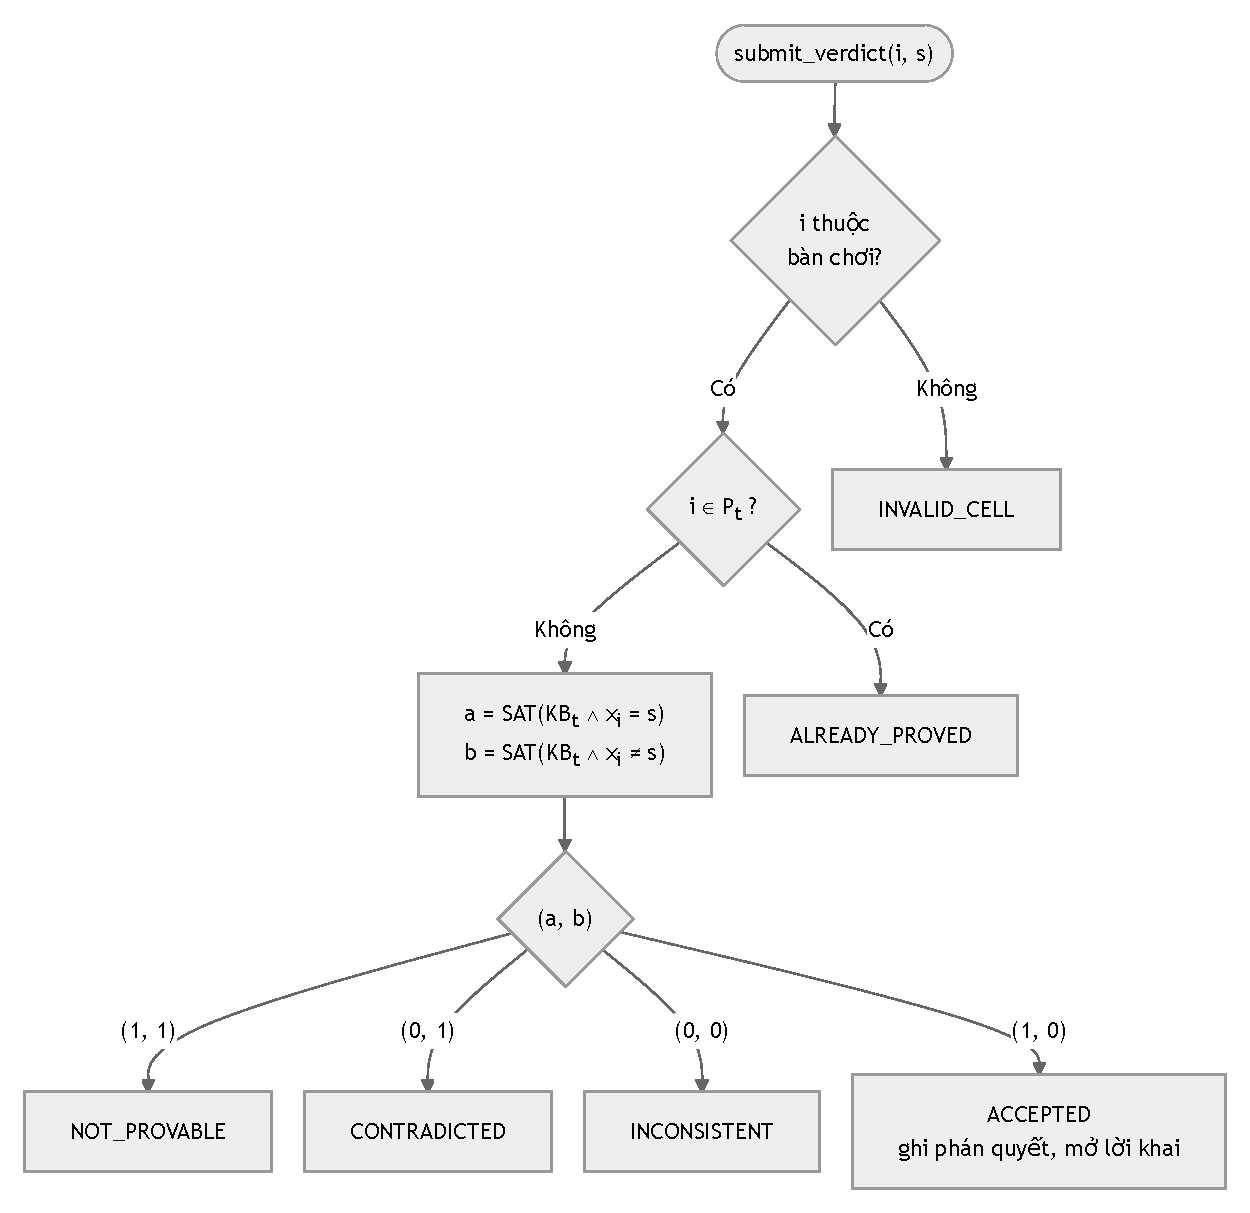
\includegraphics[width=0.78\linewidth]{figures/verdict_outcome.pdf}
  \caption{Thứ tự kiểm tra khi nộp phán quyết $\langle i, s\rangle$. Hai kiểm
    tra đầu không cần bộ giải; bốn kết quả cuối được quyết định bởi hai truy vấn
    SAT $a$ và $b$.}
  \label{fig:verdict_outcome}
\end{figure}

\begin{table}[htbp]
  \centering
  \caption{Các kết quả của \texttt{submit\_verdict}}
  \label{tab:submit_outcome}
  \begin{tabularx}{\textwidth}{ll>{\raggedright\arraybackslash}X}
    \toprule
    \textbf{Kết quả} & \textbf{Điều kiện} & \textbf{Ý nghĩa} \\
    \midrule
    \texttt{INVALID\_CELL}   & $i \notin \mathcal{C}$          & Ô không thuộc bàn chơi \\
    \texttt{ALREADY\_PROVED} & $i$ đã có trong $\mathcal{P}_t$ & Ô đã được chứng minh trước đó \\
    \texttt{ACCEPTED}        & $a \land \neg b$                & $\mathit{KB}_t \models (x_i = s)$; ghi phán quyết và lật lời khai của ô $i$ \\
    \texttt{NOT\_PROVABLE}   & $a \land b$                     & Cả hai trạng thái còn khả dĩ; chưa đủ bằng chứng \\
    \texttt{CONTRADICTED}    & $\neg a \land b$                & $\mathit{KB}_t \models (x_i \ne s)$; phán quyết sai \\
    \texttt{INCONSISTENT}    & $\neg a \land \neg b$           & $\mathit{KB}_t$ không thỏa được; bản đồ bị lỗi \\
    \bottomrule
  \end{tabularx}
\end{table}

\paragraph{Luật không đoán.}
Kết quả \texttt{NOT\_PROVABLE} hiện thực luật trung tâm của Griductive: một phán
quyết đúng với lời giải nhưng chưa được $\mathit{KB}_t$ suy ra vẫn bị từ chối.
Trò chơi gốc mô tả luật này là ``bạn không bao giờ phải đoán: tại mọi thời
điểm, luôn có ít nhất một phán quyết suy ra được từ các lời khai''
\cite{griductive_rules}. Luật có hai mặt. Về phía người chơi, mỗi phán quyết
được chấp nhận đều kèm một chứng minh, nên trò chơi là bài toán suy diễn chứ
không phải thử và sai. Về phía người thiết kế, mỗi bản đồ phải bảo đảm rằng tại
mọi trạng thái chưa hoàn thành luôn tồn tại ít nhất một ô thỏa
\eqref{eq:entailment}. Hàm \texttt{validate\_puzzle} kiểm chứng điều kiện thứ
hai bằng cách cho một người chơi hoàn hảo đi qua Game Engine thật và báo lỗi
nếu có một lượt không phán quyết nào được chấp nhận.
